\section{Miłosz Kluczek}
\label{sec:kluczek}

Dodałem zdjęcie owczarka niemieckiego (Figure~\ref{fig:owcz}).

\begin{figure}[htbp] % Co oznacza [htbp]?
    \centering
    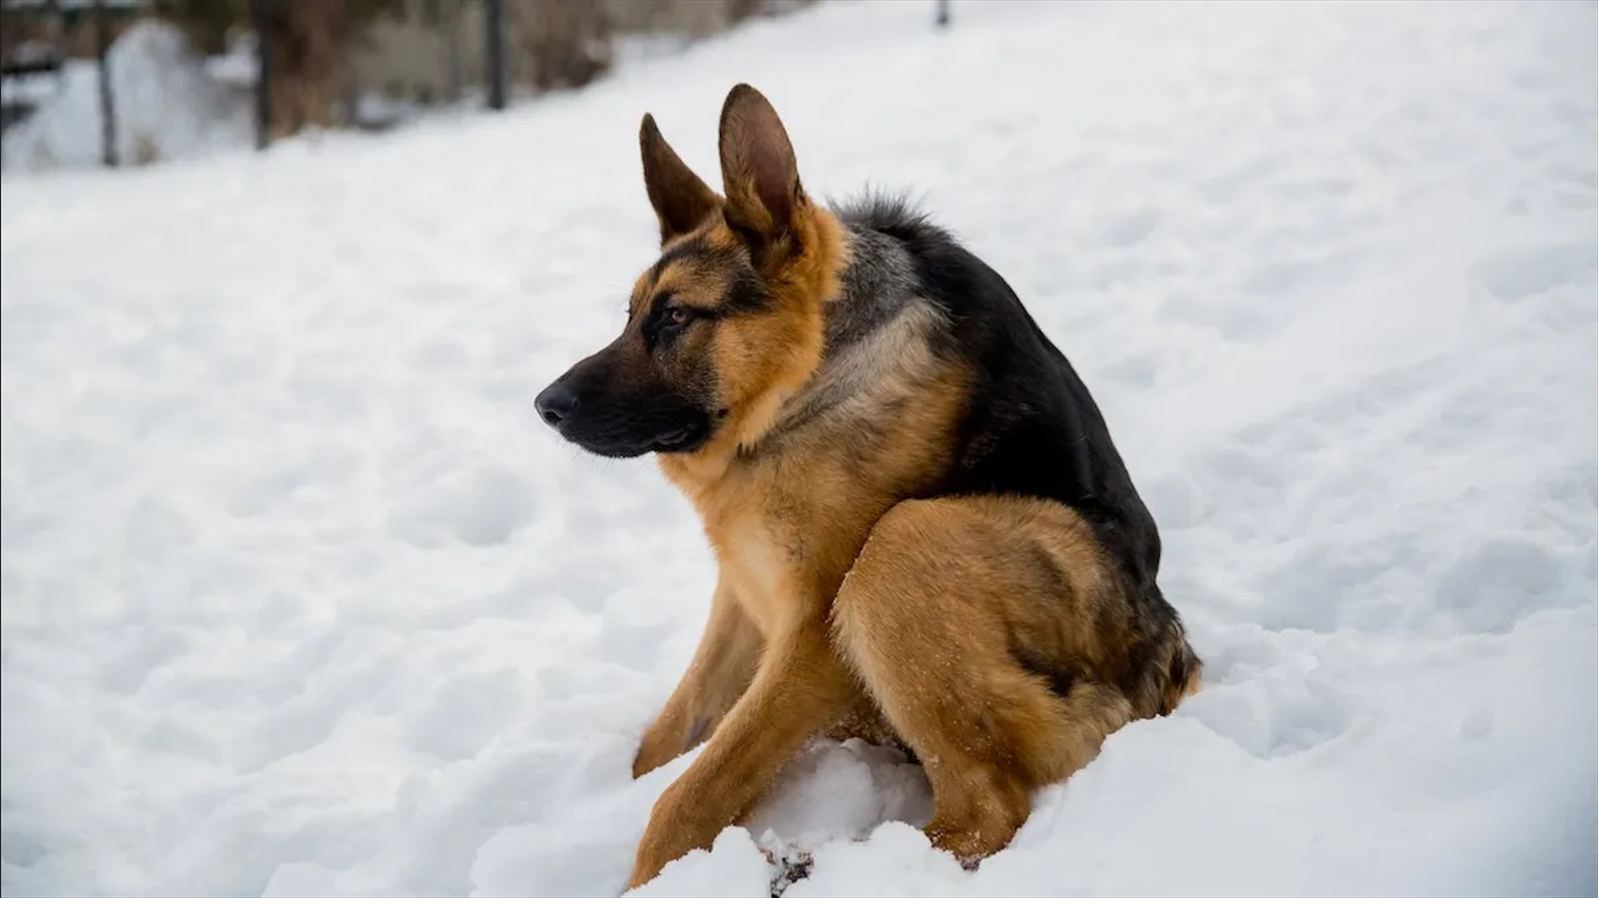
\includegraphics[width=1\textwidth]{pictures/owczarek.png} 
    \caption{Ten pies nie ma szyi.}
    \label{fig:owcz}
\end{figure}

\hline \hspace{1cm}




Tabela~\ref{tab:statki} pokazuje przykładowe rozstawienie statków w grze Statki. 

\begin{table}[htbp]
\centering
\begin{tabular}{|l|l|l|l|l|l|}
\hline
  & A & B & C & D & E \\ \hline
1 & X & X & X & X & . \\ \hline
2 & . & . & . & . & . \\ \hline
3 & X & X & X & . & X \\ \hline
4 &   &   &   &   & X \\ \hline
4 & . & X & X & . & . \\ \hline
\end{tabular}
\caption{Statki to gra strategiczno-planszowa dla dwóch osób.}
\label{tab:statki}
\end{table}

\hline \hspace{1cm}

Lista nienumerowana losowych wyrazów:
\begin{itemize}
  \item Pies
  \item Kot
  \item Długopis 
\end{itemize}

Lista numerowana losowych wyrazów:
\begin{enumerate}
    \item Poseł
    \item Minister
    \item Prezydent
\end{enumerate}

\newpage


\textbf{Pies domowy} (\textit{Canis familiaris}) – udomowiony gatunek ssaka drapieżnego z rodziny psowatych (\textit{Canidae}), traktowany przez niektóre ujęcia systematyczne za podgatunek wilka, a przez inne za odrębny gatunek, opisywany pod synonimicznymi nazwami \textit{Canis lupus familiaris} lub \textit{Canis familiaris}. Od czasu jego udomowienia powstało wiele ras, znacznie różniących się morfologią i cechami użytkowymi. Rasy pierwotne powstawały głównie w wyniku presji środowiskowej. Rasy współczesne uzyskano w wyniku doboru sztucznego.

\textbf{Mózg psa} - z powodu różnic w wielkości poszczególnych psów, mózg tych zwierząt może być różnej wielkości. W przypadku ras małych jest jednak proporcjonalnie większy w stosunku do masy ciała. Mózg tych zwierząt jest anatomicznie zbliżony do ludzkiego, aczkolwiek ośrodek odpowiadający za zmysł węchu jest o ok. \textcolor{blue}{40 procent większy}. Badania wykazały, że zwierzęta te odbierają bodźce podobnie jak ludzie, potrafiąc odczuwać radość i smutek, a nawet będąc w stanie interpretować słowa wypowiadane przez ludzi.

\hspace{1cm} \hline \hspace{1cm}
\begin{center}
\textbf{Przykładowe równanie matematyczne:}
\hspace{3cm}
$\cos (2\alpha) = \cos^2 \alpha - \sin^2 \alpha$
\end{center}